\begin{frame}
  \frametitle{Benchmark}
  \framesubtitle{Goodness Modeling}
  \monocolumn{
    \begin{tikzbenchmarkfig}{Prediction Error}
      \begin{pgfonlayer}{background}
        \node[main plot] (main){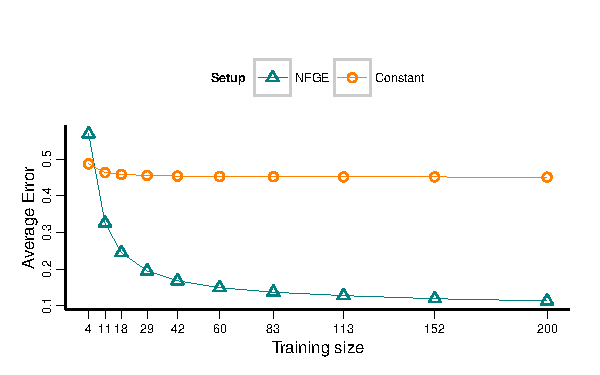
\includegraphics[trim=1.2cm 1.21cm 0.6cm 2.15cm, clip]{figures/nfge/synthetic_results.pdf}};
      \end{pgfonlayer}

      \node[below=0cm of main.south](axisx){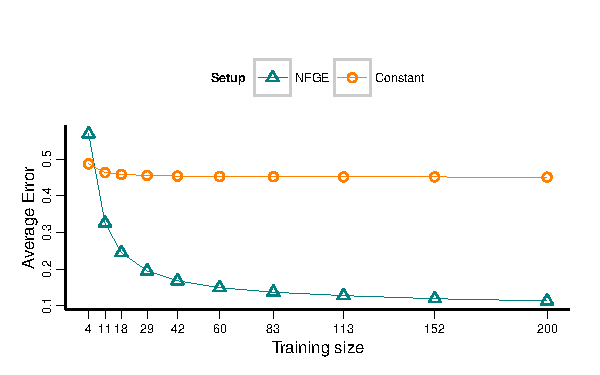
\includegraphics[trim=1.2cm 0.7cm 0.6cm 5.25cm, clip]{figures/nfge/synthetic_results.pdf}};
      \node[below=0.1cm of axisx.south]{Training Set Size};

      \node[left=0cm of main.north west,anchor=north east](axisy){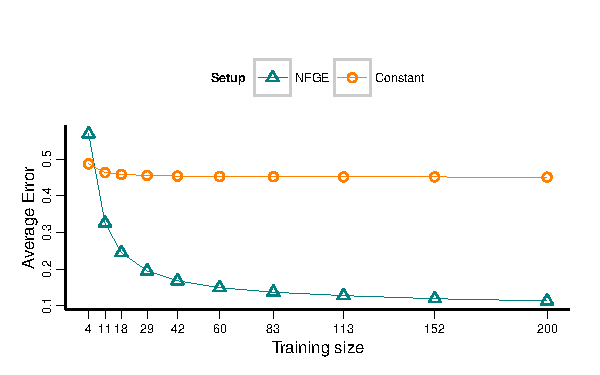
\includegraphics[trim=0.7cm 1.3cm 9.06cm 2.15cm, clip]{figures/nfge/synthetic_results.pdf}};
      \node[left=0.5cm of main.west,anchor=east]{\rotatebox{90}{Average Error}};

      \node[anchor=south,above=0.5cm of main.north] (capt){
        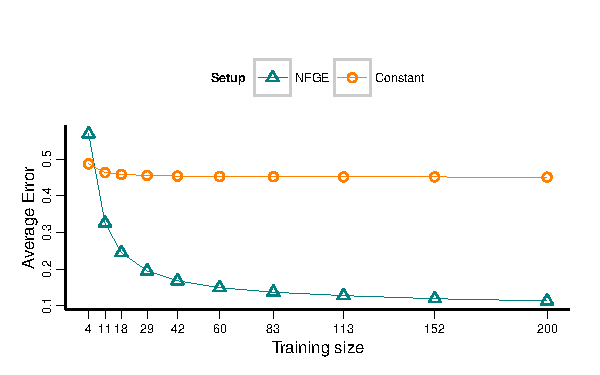
\includegraphics[trim=2cm 4.5cm 0.6cm 1cm,clip=true]
        {figures/nfge/synthetic_results.pdf}};

    \end{tikzbenchmarkfig}
  }

  \note{
    \begin{itemize}
    \item Como podem observar, ao contrario.... estimar com precisão
    \item Vemos também que o algoritmo atingiu $90\%$ da precisao
      máxima com apenas 42 observações.
    \end{itemize}

  }
\end{frame}
